\documentclass[11pt,letterpaper]{article}

%----- Configuración del estilo del documento------%
\usepackage{graphicx}
\usepackage[table]{xcolor}
\usepackage[left=2cm,right=2cm,top=1.8cm,bottom=2.3cm]{geometry}
\usepackage{fancyhdr}
\usepackage{lastpage}
\usepackage{gensymb}
\usepackage{amsmath}
\pagestyle{fancy}
\fancyhf{}
\rfoot{\textit{Página \thepage \hspace{1pt} de \pageref{LastPage}}}

%------ Paquetes matemáticos básicos --------%
\usepackage{amsmath, amssymb, amsthm}

%------ Texto aleatorio y listas ----- %
\usepackage{lipsum, enumitem}

\begin{document}

%------ Encabezado -------- %
\begin{center}
    \begin{minipage}{3cm}
    	\begin{center}
    		\includegraphics[height=3.4cm]{imagenes/logo_unam.png}
    	\end{center}
    \end{minipage}\hfill
    \begin{minipage}{10cm}
    	\begin{center}
    	\textbf{\large Universidad Nacional Autónoma de México}\\[0.1cm]
        \textbf{Facultad de Ciencias}\\[0.1cm]
        \textbf{Matemáticas para las Ciencias Aplicadas 2 | Grupo 7056}\\[0.1cm]
        \textbf{Tarea 1 }\\[0.1cm]
        Cisneros Álvarez Danjiro\\[0.1cm]
        Rodríguez López Luis Fernando\\[0.1cm]
        Tenorio Reyes Ihebel Luro\\[0.1cm]
        21/02/2025
    	\end{center}
    \end{minipage}\hfill
    \begin{minipage}{3cm}
    	\begin{center}
    		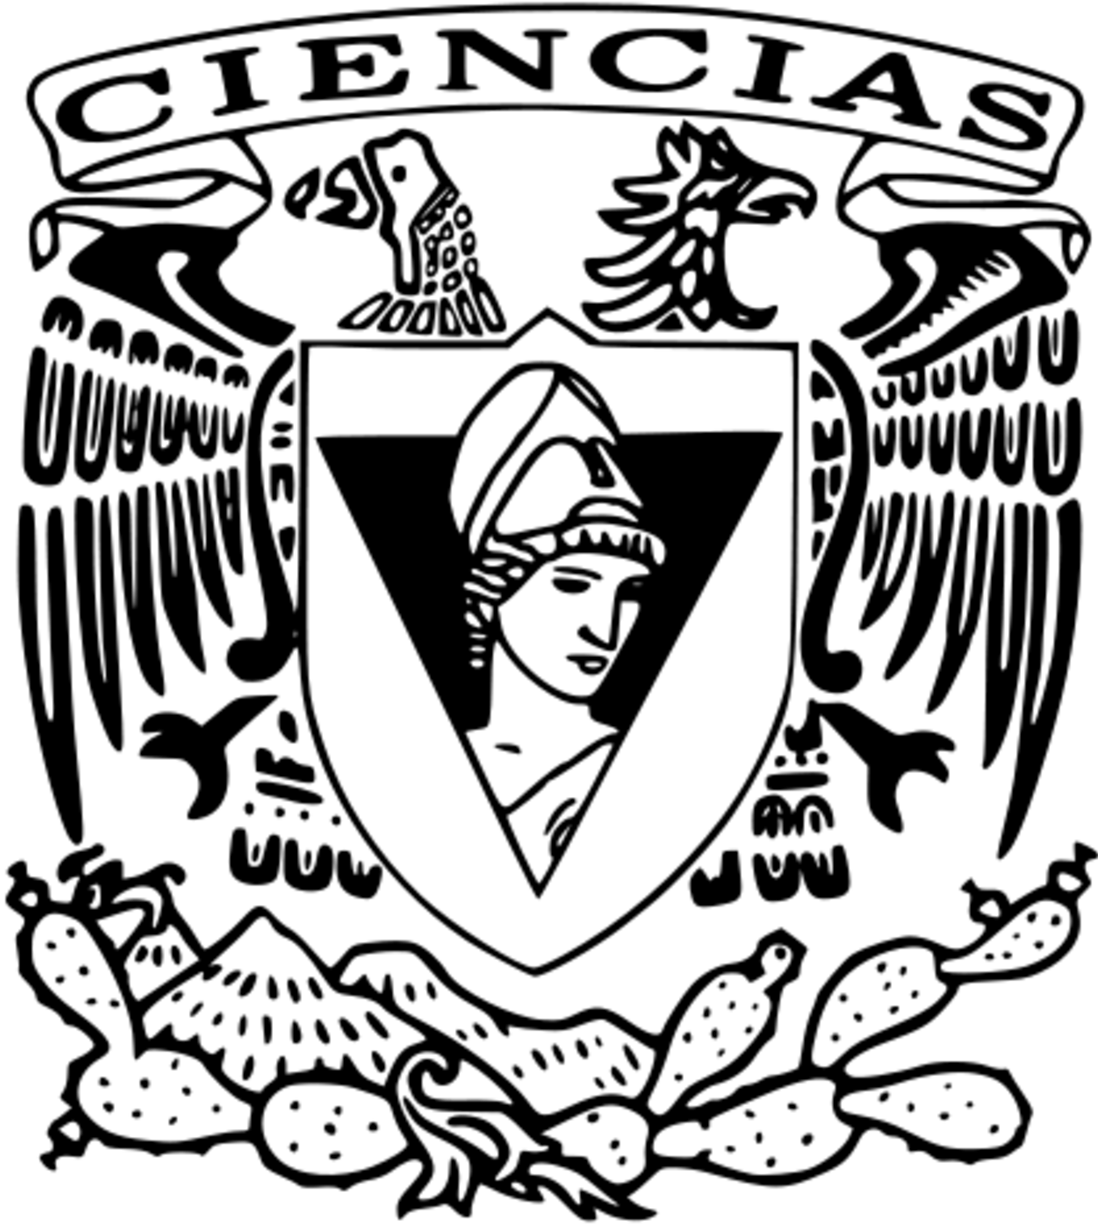
\includegraphics[height=3.4cm]{imagenes/Logo_FC.png}
    	\end{center}
    \end{minipage}
\end{center}

\noindent\rule{\linewidth}{0.4pt}

%------ Fin de encabezado -------- %

%\section*{1ra Parte}

\subparagraph{Ejercicios: Sección 11.2 Anton-Bivens-Davis (pp. 782-784).}

% ---- 01. Ejercicio 52 DANJIRO ---- %
\section{Ejercicio 52, Sección 11.2}
Se dice que una partícula esta en un equilibrio estático si la resultante de todas las fuerzas 
aplicadas es igual a cero. En estos ejercicios, encientra la furza F que debe ser aplicada al punto para producir un equilibrio estático. Describe F especificando su magnitud y el ángulo que hace respecto al eje positivo de x. 
Para resolver este ejercicio hice los siguientes pasos:
\begin{itemize}
    \item Empecé con etiquetar cada fuerza con un nombre para hacer más eficiente la solución: $F_1 = 120$N, $F_2 = 150$N y $F_3 = 100$N.
    \item Luego para sacar los vectores de cada fuerza use la longitud y ángulo de cada fuerza, medí los ángulos respecto al eje x positivo:
    \begin{equation*}
    F_1 = 135\degree, F_2 = 60\degree, F_3 = 0\degree        
    \end{equation*}
    \item Use la siguiente fórmula para cada fuerza y sacar el vector de las 3 fuerzas usando la longitud y el ángulo de estas, resolviendo la fórmula qeudaría así:
    \begin{center}
        $F_1 = 120<cos(135), sen(135)> \simeq <-84.8528, 84.8528>$
        $F_2 = 150<cos(60), sen(60)> \simeq <75, 129.9038>$
        $F_3 = 100<cos(0), sen(0)> \simeq <100, 0>$
    
    \end{center}
    \item Al ya tener todos los vectores de cadaa fuerza, sumamdos los 3 vectores para obtener las fuerza final de la combinación de las 3 fuerzas:
    \begin{center}
        $F_T = (F_1 + F_2 + F_3) = <-84.8528 + 75 + 100, 84.8528 + 129.9038 + 0> \simeq <90.1479, 214.7560>  $ 
    \end{center}
    \item Para finalizar, calculamos la fuerza equilibrante en forma de vector al pasar la suma de las fuerzas como negativas y sacamos su norma para medir la fuerza equilibrante:
    \begin{center}
        $||F_{eq}|| \sqrt{(-90.1479)^{2} + (-214.7560)^{2}} \simeq 232.9093 $
    \end{center}
    \item Y como podemos ver, la fuerza equilibrante que debe tener la partícula es de $232.9093$ para llegar a un equilibrio estático.
\end{itemize}

% ---- 02. Ejercicio 56 LUIS ---- %
\section{Ejercicio 56, Sección 11.2}
Un bloque con un peso de 100 N está suspendido por cables A y B, como se muestra en la figura adjunta.
\begin{enumerate}
    \item Utilice una herramienta gráfica para graficar las fuerzas que el bloque ejerce a lo largo de los cables A y B como funciones del ``hundimiento'' $d$.
    \item ¿El aumento del hundimiento incrementa o disminuye las fuerzas en los cables?
    \item ¿Cuánto hundimiento se requiere si los cables no pueden tolerar fuerzas superiores a 150 N?
\end{enumerate}

\begin{figure}[h]
    \centering
    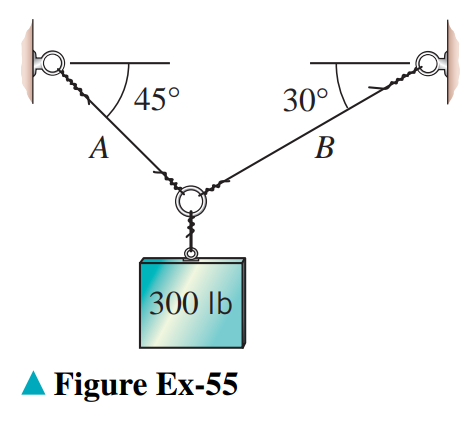
\includegraphics[width=0.2\textwidth]{imagenes/Figure_Ex-55.png}
    \hspace{5cm}
    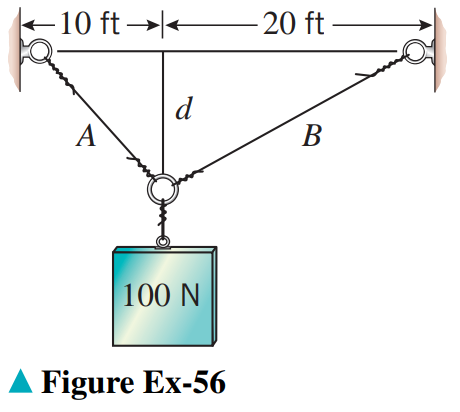
\includegraphics[width=0.2\textwidth]{imagenes/Figure_Ex-56.png}
\end{figure}


% ---- 03. Ejercicio 58 IHEBEL ---- %
\section{Ejercicio 58, Sección 11.2}
\section{Ejercicio 58, Sección 11.2}
Un vector $w$ es una combinacón lineal de los vectores $v_1$, $v_2$ y $v_3$, si $w$ puede ser expresado como una $w=c_1v_1+c_2v_2+c_3v_3$ donde $c_1$, $c_2$ y $c_3$  son escalares.\\
\textbf{a) Encuentra los escalares $c_1$, $c_2$ y $c_3$ para expresar $<-1,1,5>$ como una combinacion lineal de $v_1=<1,0,1>$, $v_2=<3,2,0>$ y $v_3=<0,1,1>$ .}\\\
Tenemos entonces lo siguiente:
\begin{equation*}
    \begin{split}
        <-1,1,5> &= c_1<1,0,1> + c_2<3,2,0> + c_3<0,1,1>\\
        &=<c_1,0,c_1> + <3c_2,2c_2,0> + <0,c_3,c_3>\\
        &=<c_1+3c_2+0,0+2c_2+c_3,c_1+0+c_3>
    \end{split}
\end{equation*}

De aqui podemos ver el siguiente sistema de ecuaciones.

\begin{equation*}
     \left\{\begin{matrix}
         c_1 + 3c_2 + 0&= -1 & (1\\
         0 + 2c_2 + c_3&= 1 & (2\\
         c_1 + 0 + c_3&= 5  & (3\\
\end{matrix}\right.
\end{equation*}

Por sustitucion:

\textit{1)}
\begin{equation*}
        c_1=-1-3c_2
\end{equation*}

\textit{2)}
\begin{equation*}
    c_3=1-2c_2
\end{equation*}

\textit{3)}
\begin{equation*}
    \begin{split}
        -1-3c_2+c_3 &= 5\\
        -1-3c_2+1-2c_2&=5\\
        -5c_2 &= 5\\
        c_2&=-1
    \end{split}
\end{equation*}
\textit{Resolvemos el resto}
\begin{equation*}
    \begin{split}
        c_3 &= 1-2(-1)\\
        c_3 &= 1+2\\
        c_3 &=\\ \\
        c_1 &= -1-3(-1)\\
        c_1 &= -1+3\\
        c_1 &= 2
    \end{split}
\end{equation*}

Por lo tanto, los escalares son $c_1=2$, $c_2=-1$ y $c_3=3$.


\textbf{b) Muestra que el vector $2\hat{i} + \hat{j} - \hat{k}$ no puede ser expresado como una combinacion lineal de $v_1=\hat{i}-\hat{j}$, $v_2=3\hat{i}+\hat{k}$, $v_3=4\hat{i}-\hat{j}+\hat{k}$}
\begin{equation*}
    \begin{split}
        <2,1,-1> &= x<1,-1,0> + y<3,0,1> + z<4,-1,1>\\
        &= <x,-x,0> + <3y,0,y> + <4z,-z,z>\\
        &= <x+3y+4z,-x+0-z,0+y+z>
    \end{split}
\end{equation*}
\begin{equation*}
     \left\{\begin{matrix}
         x+3y+4z &= 2 & (1\\
         -x+0-z &= 1 & (2\\
         0+y+z &= -1  & (3\\
    \end{matrix}\right.
\end{equation*}

Observamos rapidamente que si despejamos x de (2) y y de (3) tenemos:
\begin{equation*}
    \begin{split}
        -z-1&=x\\
        y&=-1-z
    \end{split}
\end{equation*}

Que significa que en este sistema $x=y$.

Como dos variables son iguales, tenemos que no hay solucion para el sistema y $\therefore$ el vector $2\hat{i} + \hat{j} - \hat{k}$ no es una combinacion lineal de $v_1$, $v_2$ y $v_3$



\subparagraph{Ejercicios: Sección 11.3 Anton-Bivens-Davis (pp. 792-794).}

% ---- 04. Ejercicio 19 LUIS ---- %
\section{Ejercicio 19, Sección 11.3}
La figura adjunta muestra un cubo.
\begin{enumerate}
    \item Encuentre el ángulo entre los vectores $\mathbf{d}$ y $\mathbf{u}$ al grado más cercano.
    \item Haga una conjetura sobre el ángulo entre los vectores $\mathbf{d}$ y $\mathbf{v}$, y confirme su conjetura calculando el ángulo.
\end{enumerate}

\begin{figure}[h]
    \centering
    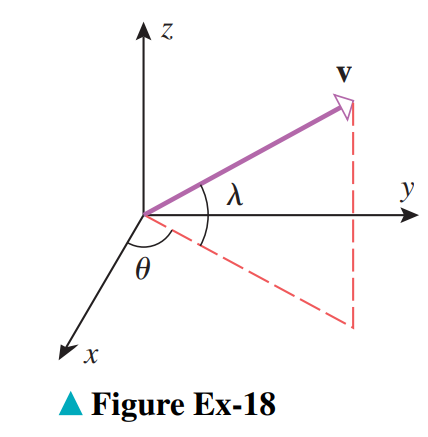
\includegraphics[width=0.2\textwidth]{imagenes/Figure_Ex-18.png}
    \hspace{5cm}
    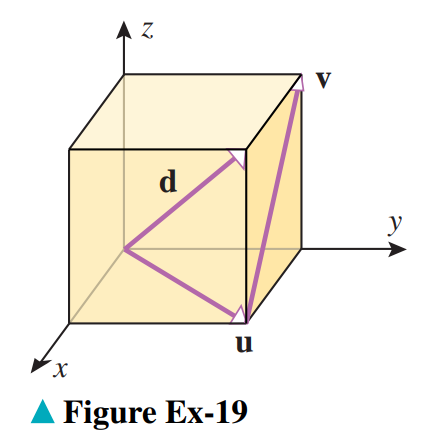
\includegraphics[width=0.2\textwidth]{imagenes/Figure_Ex-19.png}
\end{figure}


% ---- 05. Ejercicio 34 IHEBEL ---- %
\section{Ejercicio 34, Sección 11.3}
Como se muestra en la figura adjunta, un niño con masa de 34 kg está sentado en un tobogán de juegos suave (sin fricción) que está inclinado en un ángulo de $27^\circ$ con la horizontal. Estime la fuerza que el niño ejerce sobre el tobogán, y estime cuánta fuerza debe aplicarse en la dirección de $\mathbf{P}$ para evitar que el niño se deslice hacia abajo por el tobogán. Tome la aceleración debida a la gravedad como 9.8 m/s$^2$.\\


a)sea la fuerza del niño sobre la resbaladilla, sabemos que existe una fuerza con dirección hacia abajo de magnitud $(9.8)(34)=333.2N$, de ahí como el tobogan tiene un ángulo respecto a la horizontal con 27°, vemos que la fuerza se descompone en 2, una que va en sentido ortogonal al tobogán (llamémosle $F_2$) y otra en sentido paralelo que apunta a la izquierda (llamémosle $F_1$), Dadas estas condiciones:
\begin{equation*}
    \begin{split}
        333.2 &= ||G_1+G_2||\\
        ||G_1||&=||G||\cos{63\degree}\\
        &=333.2\cos{\frac{7}{20}\pi}\\
        &=151.27N\\
        ||G_2||&=||G||\sin{63\degree}\\
        &=333.2\sin{\frac{7}{20}\pi}\\
        &=296.88N
    \end{split}
\end{equation*}
$\therefore$ La fuerza que el niño ejerce sobre la resbaladilla es de 296.88N\\

b) La fuerza que lo mantiene estatico es la isma de $G_1$ pero en sentido contrario

% ---- 06. Ejercicio 35 DANJIRO ---- %
\section{Ejercicio 35, Sección 11.3}
Para el niño del Ejercicio 34, estime cuánta fuerza debe aplicarse en la dirección de $\mathbf{Q}$ (mostrada en la figura adjunta) para evitar que el niño se deslice hacia abajo por el tobogán.

\begin{figure}[h]
    \centering
    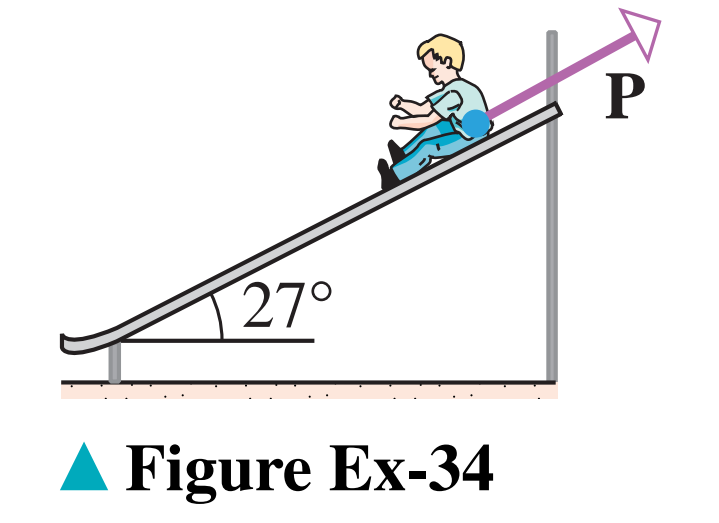
\includegraphics[width=0.2\textwidth]{imagenes/Figure_Ex-34.png}
    \hspace{5cm}
    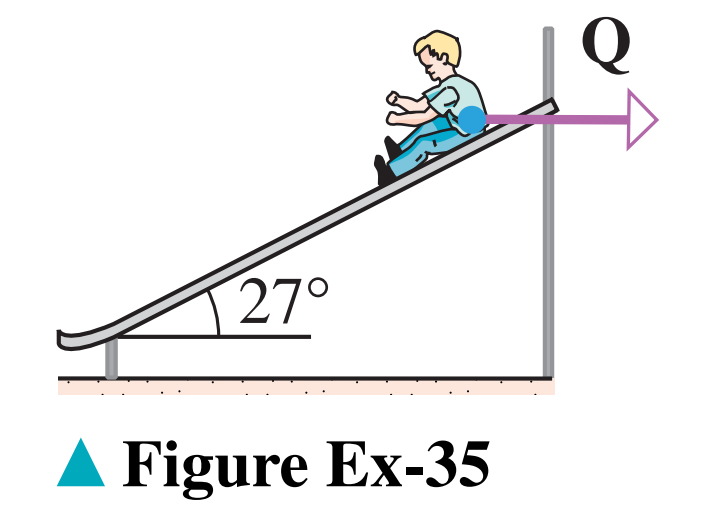
\includegraphics[width=0.2\textwidth]{imagenes/Figure_Ex-35.png}
\end{figure}

\begin{itemize}

    \item Para este ejercicio, usaremos 2 datos del punto anterior, los cuales son la fuerza aplicada hacia abajo ($333.2$) y la fuerza en diagonal hacia abajo ($296.8833$) y suando estos datos podemos proyectar un triángulo más pequeño y podemos usar un rectangulo con la fuerza contraria de Q, la cual llamaremos Q', y usando la propiedad de los ángulos usaremos un ángulo de 63\degree, y usando las razones trigonométricas podemos reemplazar los datos de la sigueinte manera:
    \begin{center}
        $sen(\theta) = C.O./H \rightarrow sen(63\degree) = Q´/F_1 \rightarrow sen(63\degree) = Q´/296.8833$
    \end{center}
    \item Y luego al despejar Q'podemos sacar el vector inverso de Q para sacar su fuerza inversa y pasamos el grado a radianes ($63\degree = 7\pi / 20$):
    \begin{center}
        $||Q´|| = 296.8833 sen(7\pi / 20) \simeq 264.5249$
    \end{center}
    \item Y para calcular la fuerza Q, simplememte debemos hacer inverso la norma de Q' y esto nos dara la fuerza necesaria que debed tener Q para evitar que el niño se deslice:
    \begin{center}
        $Q = -Q' \rightarrow -264.5249$
    \end{center}
    
\end{itemize}

% ---- 07. Ejercicio 36 LUIS ---- %
\section{Ejercicio 36, Sección 11.3}

Suponga que el tobogán en el Ejercicio 34 tiene 4 m de largo. Estime el trabajo realizado por la gravedad si el niño se desliza desde la parte superior del tobogán hasta la parte inferior.


\subparagraph{Ejercicios: Sección 11.4 Anton-Bivens-Davis (pp. 803-805).}

% ---- 08. Ejercicio 40 IHEBEL ---- %
\section{Ejercicio 40, Sección 11.4}
La siguiente figura muestra una fuerza de 1000N aplicada a la esquina de una caja.
\begin{center}
    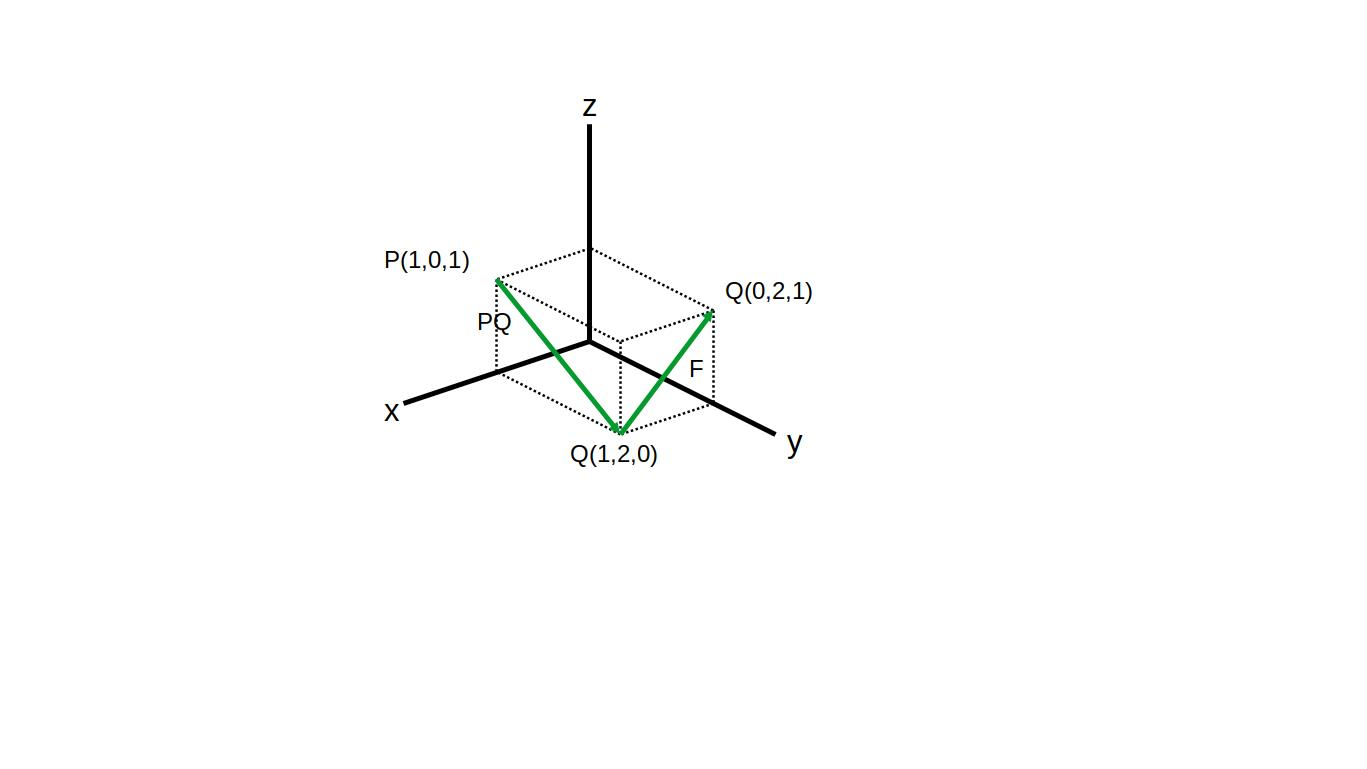
\includegraphics[height=9cm]{imagenes/Ej40.jpg}
\end{center}

\textbf{a) Encuentra el momento escalar de F sobre P}

Primero, buscamos los vectores que necesitamos
\begin{equation*}
    \begin{split}
        F &= <0-1,2-2,1-0>\\
        &= <-1,0,1>\\
        \left\| F \right\| &= \sqrt{1+1} = \sqrt{2}\\
        \left\| \hat{F} \right\| &= \left< -\frac{1}{\sqrt{2}}, 0, \frac{1}{\sqrt{2}}\right>\\
        \left\| \overrightarrow{F} \right\| &= \frac{1000}{\sqrt{2}}<-1,0,1>\\
        \left\| \overrightarrow{F} \right\| &= <1-1,2-0,0-1>\\
        &=<0,2,-1>.
    \end{split}
\end{equation*}

Ahora encontramos el momento escalar sobre P.
\begin{equation*}
    \begin{split}
        (\overrightarrow{PQ} \times \hat{F}) &=\begin{bmatrix}
            i & j & k \\
            0 & 2 & -1 \\
            -1 & 0 & 1 \\
        \end{bmatrix}\\
        &=i(2)+j(1)+k(-2)\\
        &=2i+j-2k
    \end{split}
\end{equation*}
De aqui obtenemos el torque ahora sobre P.
\begin{equation*}
    \begin{split}
        \frac{1000}{\sqrt{2}}\left\| \overrightarrow{PQ} \times \hat{F} \right\| &= \frac{1000}{\sqrt{2}}\sqrt{2^2+1^2+2^2}\\
        &=\frac{1000}{\sqrt{2}}\sqrt{4+1+4}\\
        &=\frac{1000}{\sqrt{2}}\sqrt{9}\\
        &=\frac{3000}{\sqrt{2}}
    \end{split}
\end{equation*}
Por lo tanto, el momento escalar sobre P es de $\frac{3000}{\sqrt{2}}N\cdot m$


\textbf{b) Encuentra los ángulo directores del vector momento de F sobre P al ángulo más cercano.}

Teniendo las formulas $cos\theta=\frac{\hat{v}}{||\overrightarrow{v}||}$
\begin{equation*}
    \begin{split}
        \alpha &= \arccos{\frac{2}{3}}\\
        \alpha &\approx 48\degree
    \end{split}
\end{equation*}
\begin{equation*}
    \begin{split}
        \beta &= \arccos{\frac{2}{3}}\\
        \beta &\approx 70\degree
    \end{split}
\end{equation*}
\begin{equation*}
    \begin{split}
        \gamma &= \arccos{\frac{-2}{3}}\\
        \gamma &\approx -132\degree
    \end{split}
\end{equation*}




% ---- 09. Ejercicio 41 DANJIRO ---- %
\section{Ejercicio 41, Sección 11.4}

\begin{itemize}
    
    \item Primero calcule el vector que hay entre el centro del tornillo ($\vec{F_0}$) a el punto aplicado de la fuerza ($\vec{F_1}$) usando la siguiente formula y reemplazando los vectores:
    \begin{center}
        $F_0 = (0,0)$ y $F_1 = (200, 30)$
        
        $\vec{F_0 F_1} = <200 - 0, 30 - 0>$
    \end{center}
    \item Y como la distancia esta en milimetros, debemos transformarlos en metros ya que estamos usando Newtons, por lo cual $\vec{F_0 F_1} = <0.2, 0.03>$
    \item Y ahora para sacar las coordenadas i y j del vector de $\vec{F}$ usamos la longitud y angulo de este, en este caso usamos esta fórmula y reemplazamos valores:
    \begin{center}
        $\vec{F} = \vec{||F||}<cos(\theta), sen(\theta)>$
        
        $\downarrow$
    
        $\vec{F} = 200<cos(72), sen(72)> = 200<cos(2\pi/5), sen(2\pi/5) \simeq <61.8033 i, 190.2113 j>$ 
        
    \end{center}
    \item Y ya que tenemos el vector $\vec{P_0 P_1}$ y el vector $\vec{F}$ podemos calcular su momento escalar sacando la norma del producto cruz de ambos vectores:
    \begin{center}
        $\vec{P_0 P_1} x \vec{F} = $
        
        $\begin{Bmatrix}
            0.2 & .0.03\\
            61.8033 & 190.2113
        \end{Bmatrix}$
        
    
        $\downarrow$
    
        $<38.0422 - 1.8541> $    
    \end{center}
    \item Y para terminar de sacar el momento escalar, sacamos la norma del producto cruz y nos da lo siguiente:
    \begin{center}
        $\sqrt{(38.0422)^{2} + (-1.8541)^{2}} = 38.0873 $
    \end{center}
\end{itemize}

Y por lo que podemos ver, el momento escalar de la llave inglesa es de $38.0873$ 

% ---- 10. Ejercicio 49 POR SORTEAR ---- %
\section{Ejercicio 49, Sección 11.4}
Use un CAS para aproximar el área mínima de un triángulo si dos de sus vértices son $(2, -1, 0)$ y $(3, 2, 2)$ y su tercer vértice está en la curva $y = \ln x$ en el plano $xy$.

\end{document}
